% ---------------------------------------------------------------------------- %
\subsection{Versuch 3.1 -- Spektra der R\"ohren, Analyse von LiF}
\label{subsec:spektra}
% ---------------------------------------------------------------------------- %

Der Netzebenenabstand von LiF wurde bestimmt zu:
\begin{equation*}
    d_{LiF} = \SI{204.5 \pm 0.6}{\pico\meter}
\end{equation*}

\pgfplotsset{try min ticks = 2}
\begin{figure}[ht!]
    \centering
    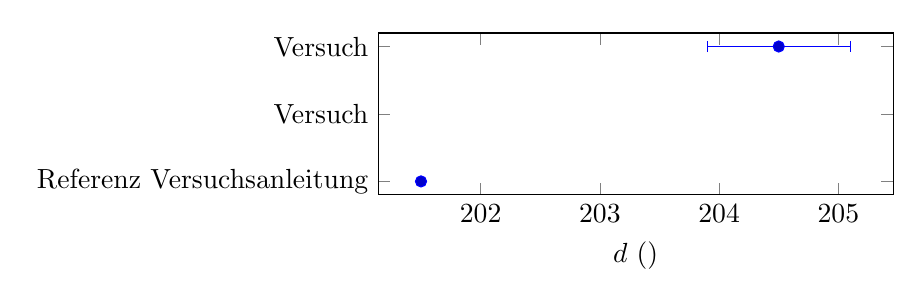
\begin{tikzpicture}
        \begin{axis}[
            width=.67\textwidth,
            height=.3\textwidth,
            %title = {Eisengehalt},
            xlabel = {$d$ ($\si{\pico\meter}$)},
            %symbolic y coords = {ungewichtet,gewichtet, QtiPlot gewichtet},
            symbolic y coords = {Referenz Versuchsanleitung,Versuch},
        ]
        \addplot+[
            only marks,error bars/.cd,
            x dir=both,x explicit,
            error bar style={line width=0.5pt},
            ]
        coordinates {
            (204.5,Versuch) +- (0.6,0)
            (201.5,Referenz Versuchsanleitung) +- (0,0)
        };
        \end{axis}
    \end{tikzpicture}
    \caption{graphische Darstellung der Ergebnisse f\"ur den Netzebenenabstand von LiF}
    \label{fig:resultsLiF}
\end{figure}

Der Referenzwert aus der Literatur ist  zwar nicht ganz im Toleranzbereich des
Experiments, aber alles  in allem betrachte ich dieses Resultat  doch als ganz
zufriedenstellend. Es w\"are  interessant, herauszufinden, ob es  genauer oder
ungenauer  ausfallen w\"urde,  wenn man  die zugeh\"orige  Funkton in  QtiPlot
direkt f\"ur zwei Variablen ($d$ und $\vartheta_0$) fitten k\"onnte.


% ---------------------------------------------------------------------------- %
\subsection{Versuch 3.3 -- Planck-Konstante}
\label{subsec:planck}
% ---------------------------------------------------------------------------- %

Die Planck-Konstante wurde experimentell bestimmt zu:
\begin{equation*}
    h_{Exp} = \SI{6.65 \pm 0.08}{\joule\second} \cdot 1e-34
\end{equation*}

Der Referenzwert aus der Literatur (Kuchling, 17. Aufl., p.526) ist:

\begin{equation*}
    h_{Ref} = \SI{6.63 \pm 0.08}{\joule\second} \cdot 1e-34
\end{equation*}

\vspace{-0.75em}
\pgfplotsset{try min ticks = 2}
\begin{figure}[ht!]
    \centering
    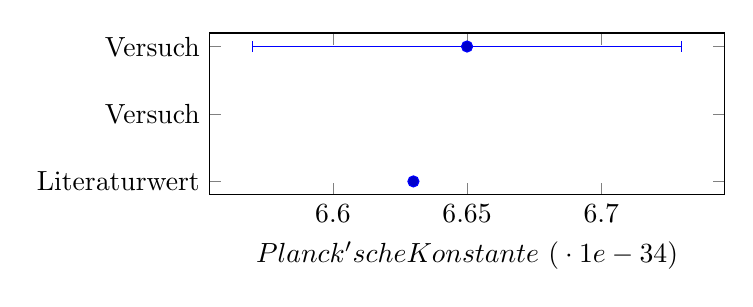
\begin{tikzpicture}
        \begin{axis}[
            width=.67\textwidth,
            height=.3\textwidth,
            %title = {Eisengehalt},
            xlabel = {$Planck'sche Konstante$ ($\si{\joule\second} \cdot 1e-34$)},
            %symbolic y coords = {ungewichtet,gewichtet, QtiPlot gewichtet},
            symbolic y coords = {Literaturwert,Versuch},
        ]
        \addplot+[
            only marks,error bars/.cd,
            x dir=both,x explicit,
            error bar style={line width=0.5pt},
            ]
        coordinates {
            (6.65,Versuch) +- (0.08,0)
            (6.63,Literaturwert) +- (0,0)
        };
        \end{axis}
    \end{tikzpicture}
    \caption{graphische Darstellung der Ergebnisse f\"ur den die Bestimmung der Planck'schen Konstante}
    \label{fig:resultsPlanck}
\end{figure}

Der  Referenzwert  liegt  innerhalb   der  Unsicherheit  des  experimentellen.
Resultates. Sehr zufriedenstellend.

\clearpage
% ---------------------------------------------------------------------------- %
\subsection{Andere Kristalle}
\label{subsec:othercrystals}
% ---------------------------------------------------------------------------- %

Die bestimmten Netzebenenabst\"ande sind:

\begin{itemize}
    \item
        \textbf{Bergkristall:}          \SI{413 \pm 3}{\pico\meter}
    \item
        \textbf{Kalkspat:}              \SI{306 \pm 6}{\pico\meter}
    \item
        \textbf{Pyrit:}                 \SI{252 \pm 0.3}{\pico\meter}
    \item
        \textbf{Synthetischer Quartz:} \SI{270 \pm 2}{\pico\meter}
\end{itemize}

Wie  im  Abschnitt  zur  Fehlerrechnung  erw\"ahnt  erachte  ich  diese  Werte
allerdings  nur  als  sehr  bedingt  aussagekr\"aftig  und  bin  der  Meinung,
dass  hier  noch   einiges  an  Arbeit  erforderlich   w\"are,  um  sinnvollte
Schlussfolderungen  ziehen  zu  d\"urfen,  die  auch  einem  kritischen  Blick
standhalten w\"urden. Leider  hat der Tag  nur 24  Stunden, und so  musste ich
hier einen  Kompromiss machen und  die Arbeit zu  Ende bringen, ohne  das Ziel
ganz erreicht zu haben.


\pgfplotsset{try min ticks = 4}
\begin{figure}[ht!]
    \centering
    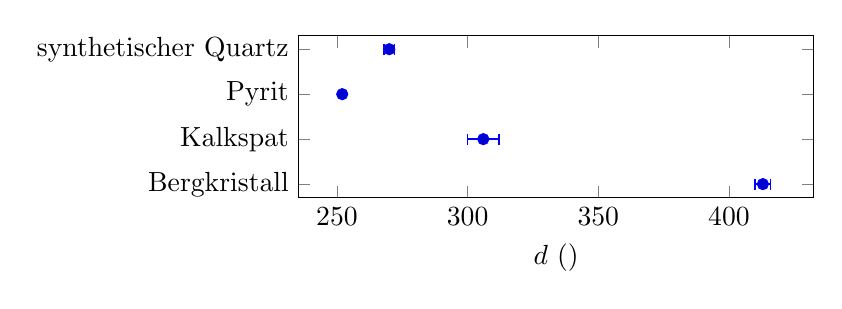
\begin{tikzpicture}
        \begin{axis}[
            width=.67\textwidth,
            height=.3\textwidth,
            %title = {Eisengehalt},
            xlabel = {$d$ ($\si{\pico\meter}$)},
            %symbolic y coords = {ungewichtet,gewichtet, QtiPlot gewichtet},
            symbolic y coords = {Bergkristall,Kalkspat,Pyrit,synthetischer Quartz},
        ]
        \addplot+[
            only marks,error bars/.cd,
            x dir=both,x explicit,
            error bar style={line width=0.5pt},
            ]
        coordinates {
            (413,Bergkristall)         +- (3,0)
            (306,Kalkspat)             +- (6,0)
            (252,Pyrit)                +- (0.3,0)
            (270,synthetischer Quartz) +- (2,0)
        };
        \end{axis}
    \end{tikzpicture}
    \caption{graphische Darstellung der Ergebnisse f\"ur den Netzebenenabstand von Bergkristall, Kalkspat, Pyrit und synthetischem Quartz }
    \label{fig:resultsOtherCrystals}
\end{figure}
